\chapter{Preliminaries}

\section{GNNs}

Consider a graph, $G = (V, E)$, or a data with graph structure. Then each node $v \in V$ is associated with a {\it node feature vector}, denoted as $X_v$.
There are two tasks of interest where GNN is commonly used:

\begin{problem}[Node Classification Problem]
Each $v \in V$ has an associated label $y_v$.

\noindent{\bf Goal:} Learn a representation vector $h_v$ of $v$ such that $y_v = f(h_v)$ i.e. such that $v$'s label can be predicted.
\end{problem}


\begin{problem}[Graph Classification Problem]
A set of graphs $\{G_1, \dots, G_N\} \subset \mathcal{G}$ is given, along with their labels $\{y_1, \dots, y_N\} \subset \mathcal{Y}$.

\noindent{\bf Goal:} Learn a representation vector $h_G$ of $G$ such that $y_G = f(h_G)$ i.e. such that $G$'s label can be predicted. 
\end{problem}


Modern GNNs follow a {\bf neighborhood aggregation strategy} (message passing strategy) in which it iteratively updates the representation of a node by aggregating representations of its neighbors.

Denote $h_v^{(k)}$ as the feature vector of node $v$ at the $k$-th iteration/layer, and let us initialize it as $h_v^{(0)} = X_v$.
Then in this framework, the $k$-th layer of a GNN can be written as

	$$a_v^{(k)} = \aggregate^{(k)} \left( \left\{ h_u^{(k - 1)} : u \in \mathcal{N}_G(v) \right\} \right)$$
	$$h_v^{(k)} = \combine^{(k)} \left( h_v^{(k - 1)}, a_v^{(k)} \right)$$

Different choices of $\aggregate^{(k)}$ and $\combine^{(k)}$ have led to different GNN variants/architectures.

\begin{architecture}[GraphSAGE\cite{Hamilton2017}]
	$$a_v^{(k)} = \MAX \left( \left\{ \relu \left( W h_u^{(k - 1)} \right) : u \in \mathcal{N}_G(v) \right\} \right)$$
	$$h_v^{(k)} = W \left[ h_v^{(k - 1)}, a_v^{(k)} \right]$$
\end{architecture}

\begin{architecture}[Graph Convolutional Networks(GCN)\cite{Kipf2017}]
	$$h_v^{(k)} = \relu \left( W \MEAN \left\{ h_u^{(k - 1)} : u \in \mathcal{N}_G(v) \cup \{v\} \right\} \right)$$
\end{architecture}


Observe that for node classification tasks, the final node representation $h_v^{(K)}$ is directly used for prediction.
However for graph classification tasks, this is not the case i.e. some additional work has to be done to "process" the final node representation to obtain the entire graph's representation.
This is done by aggregating the final node representations by $\readout$ function:
	$$h_G = \readout \left( \left\{ h_v^{(K)} : v \in V \right\} \right)$$ 
	
($\readout$ can be a simple permutation invariant function, or something more sophisticated\cite{Ying2018}\cite{Zhang2018})

%---------------------------------------------------------

\section{WL test}

Now consider the following problem:

\begin{problem}[\textsc{Graph Isomorphism (GI)}]
{\bf Input}:  Two finite graphs $G_1$ and $G_2$

\noindent{\bf Question}: $G_1 \cong G_2$?
\end{problem}

This ubiquitous problem appears everywhere: from mathematical logic, theory of computation, machine learning, to seemingly unrelated fields such as computer vision.
And this seemingly harmless problem has harassed researchers for decades!


It is currently known that \textsc{GI} can be solved in quasipolynomial time {\it i.e.} in $O \left( 2^{O \left( \left( \log n \right)^c \right)} \right) (c > 0)$ time\cite{Babai2016}.
The precise statement is as follows:
	
\begin{theorem}[Babai, 2015]
The Graph Isomorphism problem ... can be solved in quasipolynomial time.
\end{theorem}

But this is not practical.
In practice, other less efficient algorithms are used, such as algorithms by McKay (1981), Schmidt \& Druffel (1976), Ullman (1976)...etc.


Here, we shall talk about one specific combinatorial algorithm for \textsc{GI}: the Weisfeiler-Lehman test of graph isomorphism\cite{Weisfeiler1968}, or simply WL test.

WL test is proved to be successful (and computationally efficient) in isomorphism testing for a broad class of graphs\cite{Babai1979} There are some (corner) cases (ex. regular graphs) when the WL test fails\cite{Cai1992}.

The reason the people working on GNNs got so interested in the WL test is that its 1-dimensional form (a.k.a. "na\"ive vertex refinement") is {\it based on neighbor aggregations}, analogous to the GNNs!
(And that is why we'll be focused only on the 1-dim case)

Let $(G, l)$ be a labeled graph i.e. a graph $G$ with an endowed node coloring $l : V(G) \rightarrow \Sigma$.
($\Sigma$: arbitrary codomain)
Here is the full algorithm for the 1-dim WL test\cite{Shervashidze2009}:

\begin{figure}[hbt]
\centering
	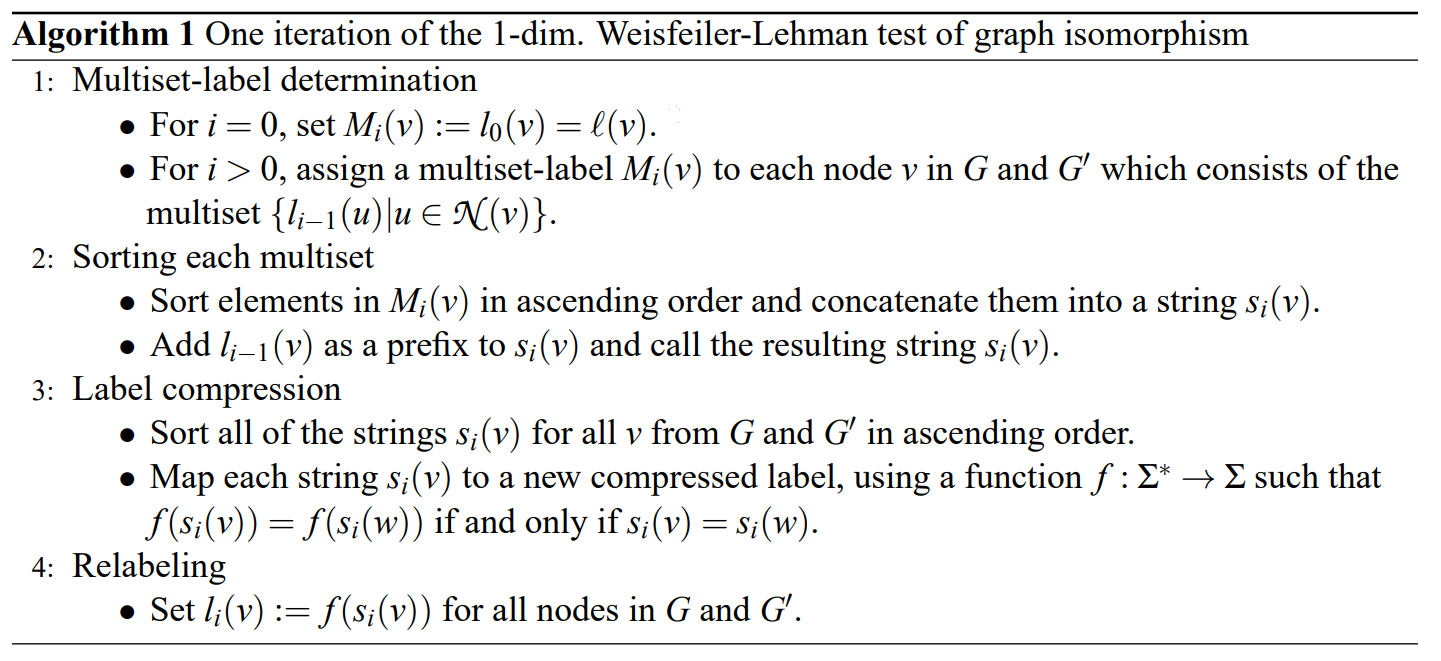
\includegraphics[height=7cm]{preliminaries/fig/wl-alg.png}
	\caption{One iteration of 1-dim WL test}
\end{figure}
	(This why this 1-dim version is commonly called the {\it color refinement algorithm})

To relate this to GNN, we need one more concept; graph kernel.

Graph kernel is a kernel function that defines {\it inner product on graphs} \cite{Vishwanathan2010}.
Intuitively, it is a function that measures the similarity of a pair of two given graphs.
There are many different variants of graph kernels, but we'll be focused on the Weisfeiler-Lehman subtree kernel\cite{Shervashidze2009}.
(Refer to \cite{Vishwanathan2010} for a extensive study of graph kernels and \cite{Shervashidze2011} for a more thorough explanation of the WL subtree kernel)

The WL subtree kernel counts common {\it original and compressed labels} i.e. common multiset strings in two graphs, resulting from 1-dim WL test.
Below shows the algorithm for calculating the WL subtree kernel:

\begin{figure}[hbt]
\centering
	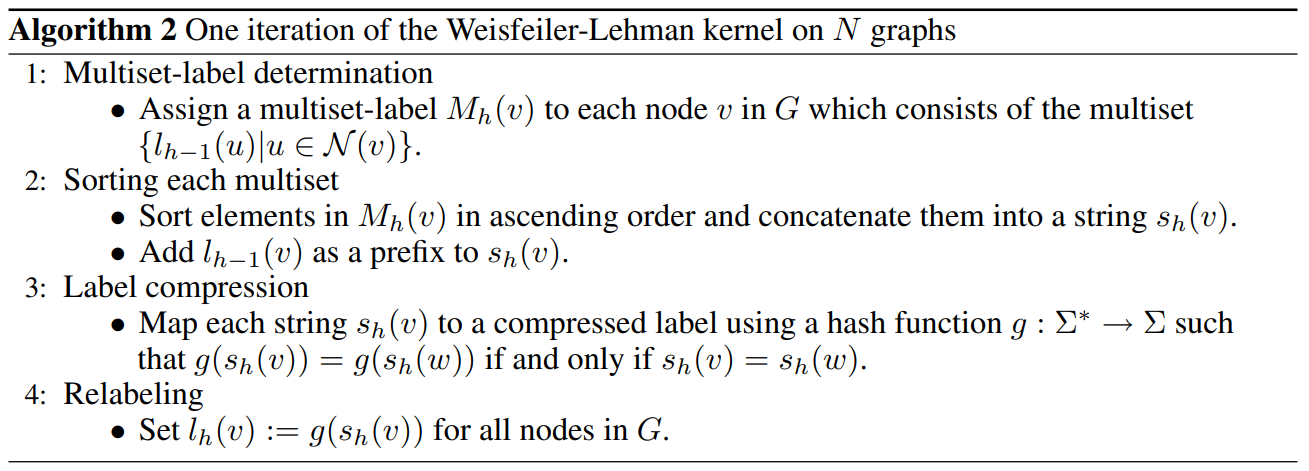
\includegraphics[height=6cm]{preliminaries/fig/wl-kernel-alg.png}
	\caption{One iteration of WL subtree kernel}
\end{figure}

And below figure is a visualization of one run of the WL subtree kernel:

\begin{figure}[hbt!]
\centering
	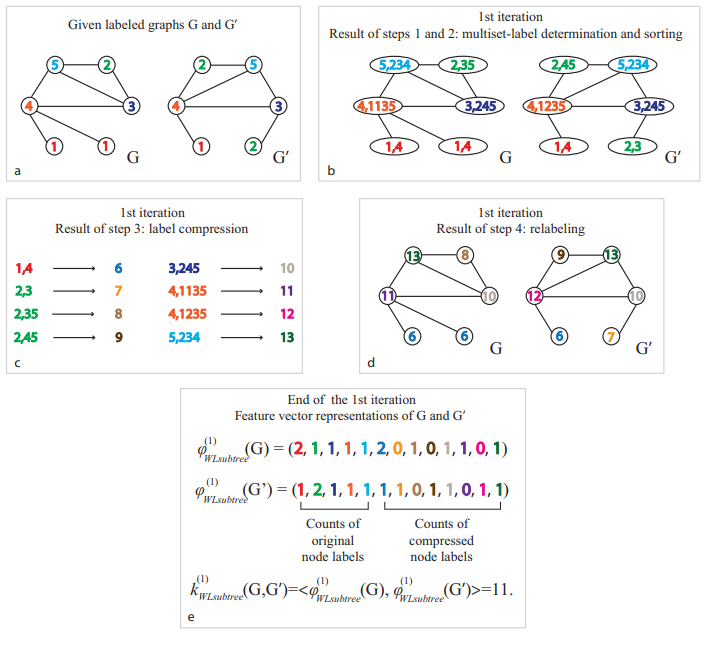
\includegraphics[height=13cm]{preliminaries/fig/fig1.png}
	\caption{Illustration of the computation of the WL subtree kernel (with respect to one iteration) for two graphs}
\end{figure}

\newpage
\section{(Overview of) Theoretical Framework}

In other words, the WL subtree uses the counts of node labels at different iterations of the WL test as the feature vector of a graph.
Intuitively, a node’s label at the $k$-th iteration of the 1-dim WL test represents a {\bf subtree structure of height k rooted at the node}.

Thus, the graph features considered by the WL subtree kernel are essentially counts of different rooted subtrees in the graph!

\begin{figure}[hbt!]
\centering
	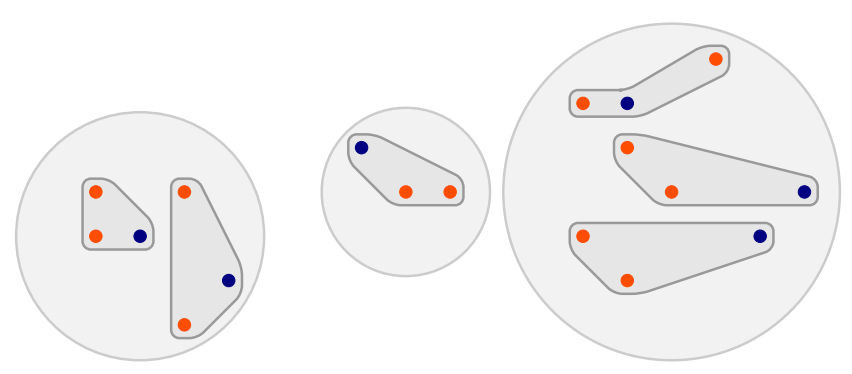
\includegraphics[height=4cm]{preliminaries/fig/fig2.png}
	\caption{An overview of the theoretical framework}
\end{figure}

What this tells us is that if a GNN's aggregation function captures the {\it full multiset} of node neighbors, the GNN can capture the rooted subtrees in a recursive manner and be as powerful as the WL test (as shown in above figure).

To analyze the representational power of a GNN, we ask ourselves the question: {\it when does a GNN map two nodes to the same location in the embedding space)? }
{\bf Intuitively, a maximally powerful GNN maps two nodes to the same location only if they have identical subtree structures with identical features on the corresponding nodes.}
Since subtree structures are defined recursively via node neighborhoods (above figure), we can reduce our analysis to the question whether a GNN maps two neighborhoods (i.e., two multisets) to the same embedding or representation.
A maximally powerful GNN would never map two different neighborhoods, i.e., multisets of feature vectors, to the same representation.
This means its aggregation scheme must be injective. Thus, we abstract a GNN’s aggregation scheme as a class of functions over multisets that their neural networks can represent, and analyze whether they are able to represent injective multiset functions.

(Above paragraph is taken directly from the paper because it is the key point in this whole work!)
